\documentclass[12pt]{article}

% Package for encoding and language support
\usepackage{indentfirst}

% \usepackage[utf8]{inputenc}
\usepackage{amsmath}
\usepackage{amssymb}
\usepackage{amsfonts}
\usepackage{geometry}
\usepackage{graphicx}
\usepackage{fancyhdr}
\usepackage{enumitem}
\usepackage{hyperref}
\usepackage{url}

% Page margins
\geometry{a4paper, margin=1in}

% Header and footer
\setlength{\headheight}{14.49998pt}
\addtolength{\topmargin}{-2.49998pt}

\pagestyle{fancy}
\fancyhf{}
\fancyhead[L]{Big-Data-Analytics HW 01}
\fancyhead[R]{Yushan Liu 2024214103}
\fancyfoot[C]{\thepage}

% Title information

\begin{document}

\begin{titlepage}
    \begin{center}
        % Insert logo
        
\includegraphics[width=5cm]{tsinghua_logo.png}\\[4cm]  % 插入图标并设置下方间距
        {\Huge Homework 1:ANOVA} \\[2cm]
        {\large Yushan Liu  \ \  Student ID: 2024214103}\\[6cm]
        {\normalsize \today}\\[1cm]
        \vfill
        \textbf{Tips}: The details of the code mentioned can be found in the attached code file \texttt{Task.ipynb}.
    
    \end{center}
\end{titlepage}

\section*{Problem 1}

One-way ANVOA is based on the following assumptions:

\begin{enumerate}
    \item \textbf{Independence of Observations}: The observations within each group and between groups must be independent of each other.
    
    \item \textbf{Normality}: The dependent variable should be approximately normally distributed for each group.
    
    \item \textbf{Homogeneity of Variances (Homoscedasticity)}: The variance of the dependent variable should be equal across the different groups being compared.
\end{enumerate}

\section*{Problem 2}

We are asked to determine if the feature "Average Age" (Col[7]) significantly varies across different group categories (Col[2]). To achieve this, we need to state the null and alternative hypotheses.

\begin{itemize}
    \item \textbf{Null Hypothesis (H$_0$)}: The average age is the same across all group categories. Mathematically, this can be written as:
    \[
    H_0: \mu_1 = \mu_2 = \mu_3 = \mu_4 = \mu_5
    \]
    Where $\mu_i$ represents the mean of the average age for category $i$ (where $i = 1, \dots, 5$).
    
    \item \textbf{Alternative Hypothesis (H$_1$)}: At least one group category has a significantly different average age compared to the others. This is expressed as:
    \[
    H_1: \exists \, i, j \ \text{such that} \ \mu_i \neq \mu_j
    \]
    This means that not all the category means are equal; at least one category has a different mean average age.
\end{itemize}

The goal of ANOVA is to test whether the null hypothesis can be rejected, indicating that there is a significant difference in the average age across the different group categories.


\section*{Problem 3}

\subsection*{(a) Empirical PDF and Normality Test}

We use the following Python code to plot the empirical probability density function (PDF) of the "Average Age" (Col[7]) and perform the Shapiro-Wilk test to assess the normality of the data:

\begin{verbatim}
    data = pd.read_excel('data.xlsx') # Load data from Excel file
    col_7 = data.iloc[:, 6]  

    sns.kdeplot(col_7, bw_adjust=0.5)
    # Plot Here()
    statistic, p_value = stats.shapiro(col_7) 

    if p_value > alpha: # alpha is the significance level (e.g., 0.05)
        print("Fail to reject null hypothesis.")
    else:
        print("Reject null hypothesis.")

\end{verbatim}

In this code, we first load the data from the Excel file and extract the "Average Age" column (Col[7]). We then plot the empirical PDF of the data using a kernel density estimate (KDE) plot. Finally, we perform the Shapiro-Wilk test to assess the normality of the data. The test outputs the test statistic and p-value, which we use to determine whether the data is normally distributed. The test normality by plot is as follows:

\begin{figure}[h]
    \centering
    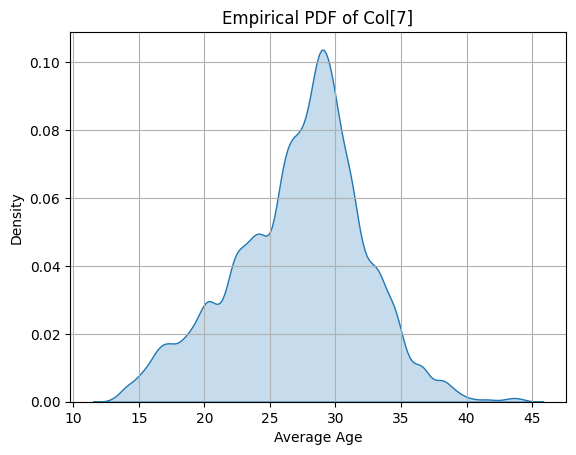
\includegraphics[width=0.68\textwidth]{image/output1.png}  
    \label{fig:Output for Normality Test}
\end{figure}

According to the Shapiro-Wilk test, the p-value is less than 0.05, indicating that we reject the null hypothesis of normality. Therefore, the "Average Age" data does not follow a normal distribution.

\subsection*{(b) Normality and Homogeneity of Variance Tests}

For each category (i = 1, ..., 5), the Shapiro-Wilk test is applied to assess the normality of the data within that category. If the p-value from the test is greater than 0.05, we cannot reject the null hypothesis, meaning the data appears to follow a normal distribution. Otherwise, the data does not follow a normal distribution.
By running the code, we can know that except the category 3, even if in the same category, the data does not follow a normal distribution.

\begin{verbatim}
    # Spilt data by category, return `average_age_by_category` as a list of arrays.
    for i, group_data in enumerate(average_age_by_category, start=1):
        shapiro_result = stats.shapiro(group_data)
        if shapiro_result.pvalue < alpha:
            print(f"Category {i} does not obey a normal distribution")
        else:
            print(f"Category {i} seems to obey a normal distribution")
\end{verbatim}


The Levene's test is performed to check the homogeneity of variances across the five categories. A p-value greater than 0.05 indicates that the assumption of equal variances holds, while a smaller p-value suggests significant variance differences between categories.
By running the code, we can know that the homogeneity of variances is not assumed.
\begin{verbatim}
    levene_test_result = stats.levene(*average_age_by_category)
    if levene_test_result.pvalue > alpha:
        print("Homogeneity of variances is assumed.")
    else:
        print("Homogeneity of variances is not assumed.")
\end{verbatim}

\subsection*{(c) One-Way ANOVA Test}

We utilized the ordinary least squares (OLS) method to define the ANOVA model, where the average age (Column 6) was treated as the dependent variable, and the category (Column 1) was the independent variable.


\begin{verbatim}
    model = ols('data.iloc[:, 6] ~ C(data.iloc[:, 1])', data=data).fit()
    anova_result = anova_lm(model)
\end{verbatim}
The ANOVA results, specifically the p-value (PR(>F)), were examined to test the null hypothesis that the average age does not vary significantly across categories.

\begin{verbatim}
    if anova_result['PR(>F)'].iloc[0] < alpha:
        print("Significant difference between the means of the groups.")
    else:
        print("No significant difference between the means of the groups.")
\end{verbatim}

A boxplot was generated to visualize the distribution of average age across different categories. We can see that there has a significant differences in average age between categories

\begin{figure}[h]
    \centering
    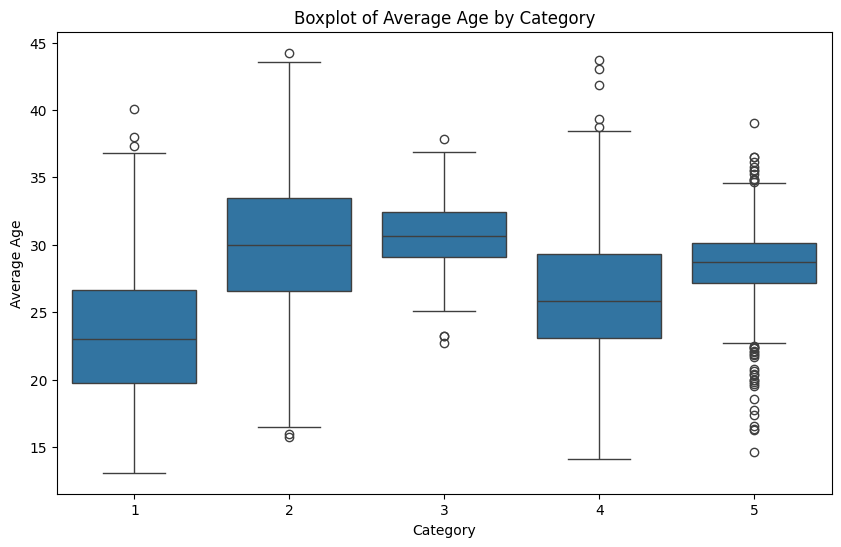
\includegraphics[width=0.65\textwidth]{image/output2.png}  
    \label{fig:Output for ANOVA test}
\end{figure}

\newpage
\section*{Problem 4}
The analysis was carried out on three key columns: \textbf{Group Size, Message Count, and Sex Ratio}.

First, we perform a normality testing for each three columns by using the Shapiro-Wilk test. 
\begin{verbatim}
    for col_index in columns_to_analyze:
        normality_result = stats.shapiro(col_data)
        if normality_result.pvalue < alpha:
            print("Do not following the normal distribution")
        else:
            print("Following the normal distribution")
\end{verbatim}

To address non-normal distributions, we applied a log transformation to each feature and then repeated the Shapiro-Wilk test. This transformation helps reduce skewness and potentially brings the data closer to a normal distribution.
\begin{verbatim}
        log_data = np.log(col_data + 1)  
        log_normality_result = stats.shapiro(log_data)
        if log_normality_result.pvalue < 0.05:
            print("Its log transformation does not obey the normal distribution")
        else:
            print("Its log transformation obey the normal distribution")
\end{verbatim}

Then we plotted the histograms of the original and log-transformed data separately as follows.We can see that neither the raw data nor the log-transformed data conform to a normal distribution.

\begin{figure}[h]
    \centering
    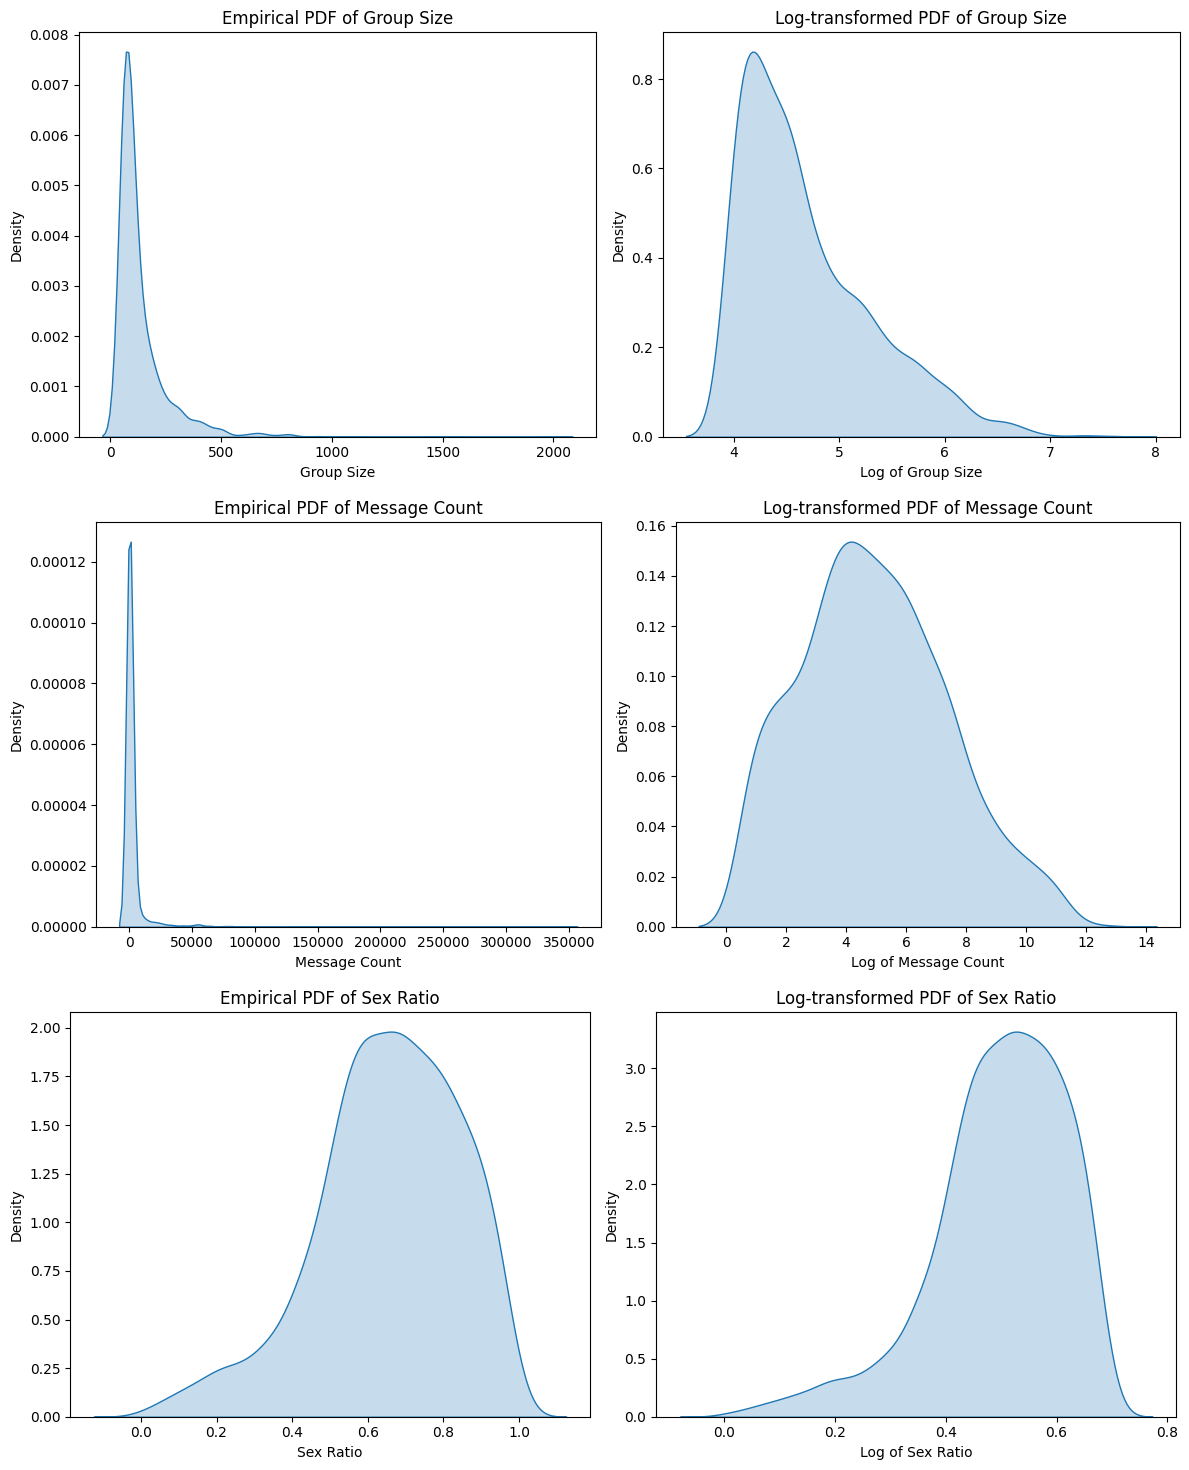
\includegraphics[width=0.8\textwidth]{image/output3.png}  
    \label{fig:PDF of Original and Log-transformed Data}
\end{figure}
\newpage

\section*{Problem 5}

\subsection*{(a) Alternative Methods for One-Way ANOVA with Non-Normal Data}

When the data does not meet the normality assumption, we can use non-parametric tests as alternatives to one-way ANOVA. Here are some alternative methods:

\begin{itemize}
    \item \textbf{Kruskal-Wallis H Test}: A rank-based test that evaluates whether the medians of two or more groups are different. It is commonly used when data is not normally distributed.
    \item \textbf{Box-Cox or Yeo-Johnson Transformation}:  Data transformations can sometimes bring the data closer to a normal distribution, allowing for a standard ANOVA.
    \item \textbf{Welch’s ANOVA}: A modified ANOVA that does not require equal variances and is less sensitive to violations of normality.
    \item \textbf{Permutational ANOVA}: Uses permutation methods to calculate p-values, making it robust to non-normal data.
\end{itemize}

\subsection*{(b) Kruskal-Wallis H Test Implementation}

To minimize the effects of skewness and extreme values, we applied a log transformation to each feature before performing the Kruskal-Wallis H test. 

\begin{verbatim}
    kruskal_result = stats.kruskal(*log_column_data)
    print("Kruskal-Wallis H Test Result:")
    print(kruskal_result)

    if kruskal_result.pvalue < alpha:
        print("Significant differences among the log-transformed feature columns.")
    else:
        print("No significant differences among the log-transformed feature columns.")

\end{verbatim}

To illustrate the distribution of each feature before and after log transformation, we plotted boxplots for both the original and log-transformed data.

We can see that the Kruskal-Wallis H test results indicate significant differences among the log-transformed feature columns.
\newpage
\begin{figure}[h]
    \centering
    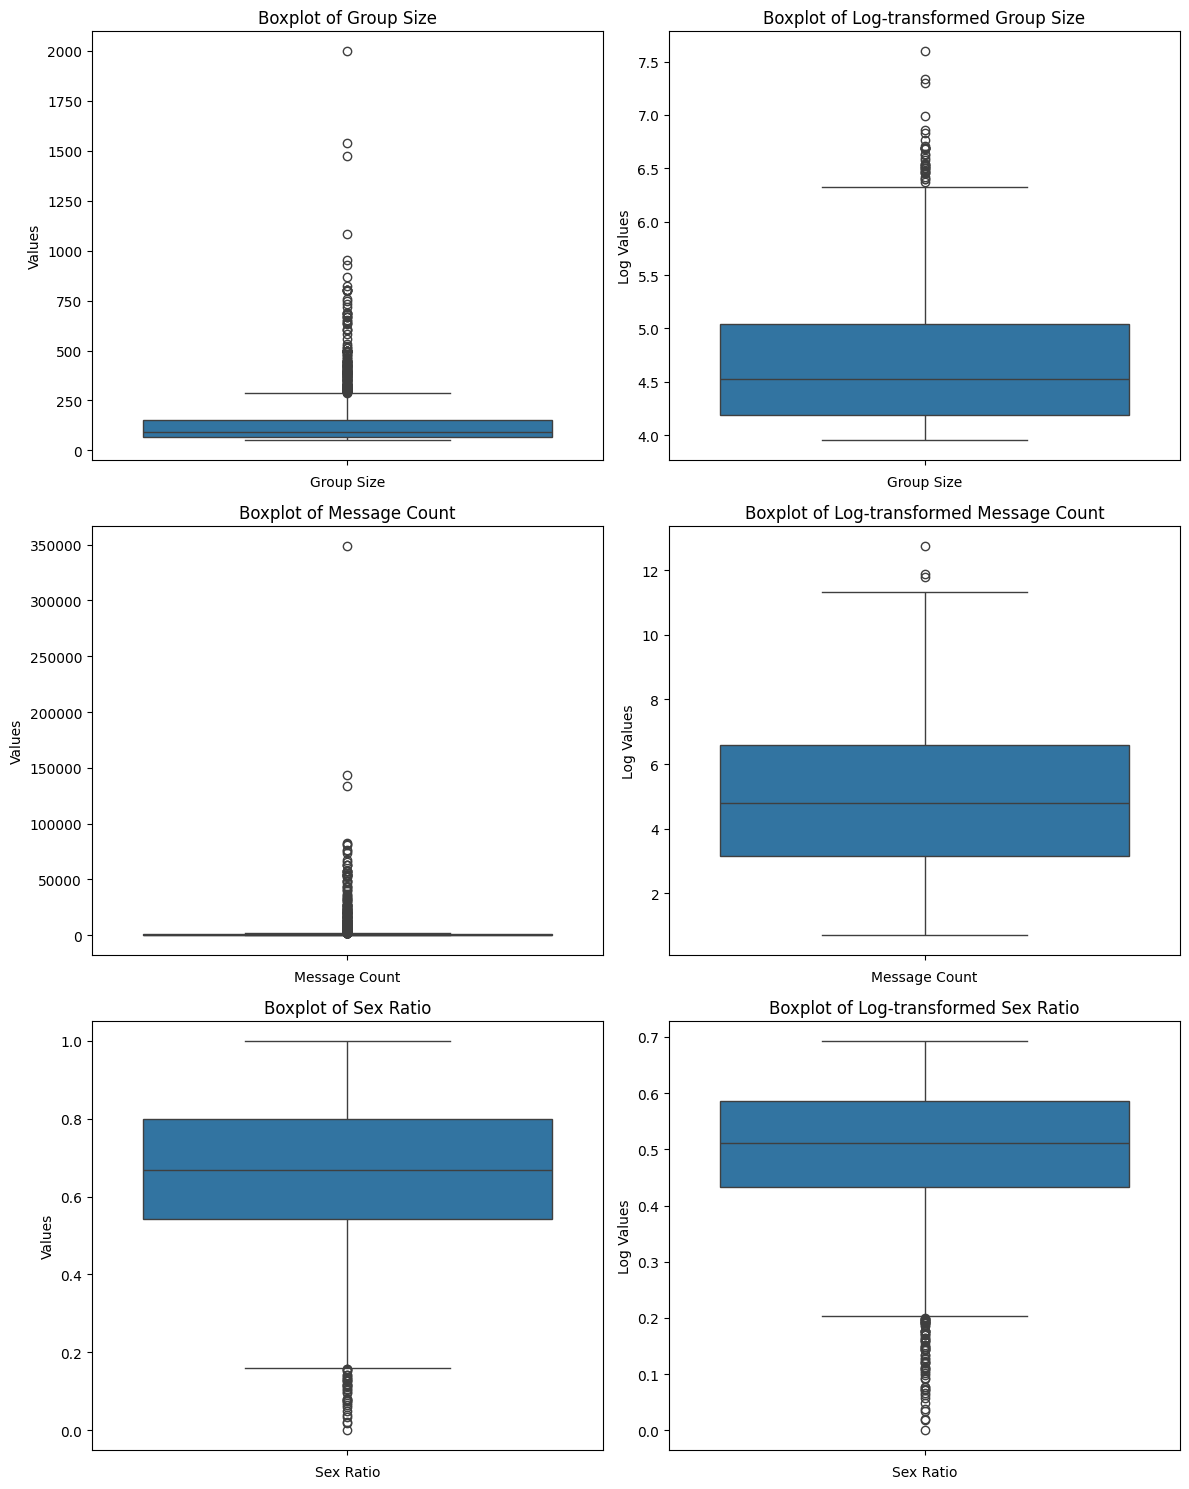
\includegraphics[width=0.8\textwidth]{image/output4.png}  
    \label{fig:Boxplot of Original and Log-transformed Data}
\end{figure}

\newpage
\begin{thebibliography}{99}

    \bibitem{seaborn}
    Waskom, M. L. (2021). Seaborn: statistical data visualization. \emph{Journal of Open Source Software}, 6(60), 3021. Available: https://doi.org/10.21105/joss.03021.
    
    \bibitem{statsmodels}
    Seabold, S., Perktold, J. (2010). Statsmodels: Econometric and statistical modeling with python. In \emph{9th Python in Science Conference} (pp. 92-96). Available: https://conference.scipy.org/proceedings/scipy2010/pdfs/seabold.pdf.
    
    \bibitem{kruskalwallis}
    Kruskal, W. H., Wallis, W. A. (1952). Use of ranks in one-criterion variance analysis. \emph{Journal of the American Statistical Association}, 47(260), 583-621. Available: https://doi.org/10.1080/01621459.1952.10483441.
    
    \bibitem{anova}
    Fisher, R. A. (1925). Statistical Methods for Research Workers. \emph{Edinburgh: Oliver and Boyd}.
    
    \bibitem{openai_chatgpt}
    OpenAI. (2024). ChatGPT: Language model for interactive support in scientific research. Available: https://openai.com/chatgpt.
    
\end{thebibliography}
    
\textbf{Tips}: The details of the code can be found in the attached code file \texttt{Task.ipynb}.
    
\end{document}   
